\documentclass[a4paper,12pt]{article}

%PACKAGES

\usepackage[utf8]{inputenc}
\usepackage[slovak]{babel}
\usepackage{comment}


\usepackage{graphicx,amsmath,amssymb, amsthm, multicol}
\usepackage{pdfpages}

\usepackage[nottoc]{tocbibind}
\usepackage{mathrsfs}
\usepackage{psfrag}
\usepackage[small,bf]{caption}
\usepackage{ifthen}

\newtheorem{defin}{Definícia}[section]
\newtheorem{theorem}[defin]{Veta}
\newtheorem{prop}[defin]{Tvrdenie}
\newtheorem{lema}[defin]{Lema}
\newtheorem{cor}[defin]{Dôsledok}
\newtheoremstyle{comment}{}{}{}{}{}{:}{ }{#1}
\theoremstyle{comment}
\newtheorem{com}{\textit{Poznámka}}

\usepackage{hyperref}                                     
\hypersetup{%  http://www.tug.org/applications/hyperref/
bookmarksnumbered,
pdfstartview={FitH},
linkcolor=black,
citecolor=black,
colorlinks=true,
pdfpagemode={None},
plainpages=false
}%

%%\usepackage{fullpage}
%%\setlength{\topmargin}{-0.5cm}
%%\setlength{\headheight}{0cm}
%%\setlength{\headsep}{0in}
\setlength{\textheight}{24cm}
\setlength{\textwidth}{15.5cm}
\addtolength{\voffset}{-1.2cm}
\addtolength{\hoffset}{-0.3cm}
%%\addtolength{\rightmargin}{-1cm}
\setlength{\parindent}{0.5cm}
\setlength{\parskip}{0in}
\linespread{1.5}



\begin{document}

  \thispagestyle{empty}
\begin{center}
{\large \bf UNIVERZITA KOMENSKÉHO V BRATISLAVE \\
FAKULTA MATEMATIKY, FYZIKY A INFORMATIKY}
\end{center}
%\begin{titlepage}
%    \rmfamily
%    \begin{center}
%      \LARGE\scshape
%      \theuniversity\\
%      \Large\upshape
%      \thefaculty\\
%      \large
%      \thedepartment
%    \end{center}
%

\vspace{2cm}
\begin{figure}[!h]
   \centering
     %
\includegraphics[width=3.5cm]{logoUK.jpg}
\end{figure}

\vspace{1cm}
\begin{center}
{\large \bf Riadkovo-stĺpcové návrhy štatistických experimentov \\
\vspace{3cm}
BAKALÁRSKA PRÁCA}
\end{center}

\vfill
%
\begin{multicols}{2}
{\bf
\begin{flushleft} 2020 \end{flushleft}
\begin{flushright} Róbert Druska \end{flushright} 
}
\end{multicols}


  \newpage
\thispagestyle{empty}
\begin{center}
{\large UNIVERZITA KOMENSKÉHO V BRATISLAVE \\
FAKULTA MATEMATIKY, FYZIKY A INFORMATIKY}
\end{center}


\vspace{5cm}
\begin{center}
{\large \bf Riadkovo-stĺpcové návrhy štatistických experimentov \\
\vspace{3cm}
BAKALÁRSKA PRÁCA}
\end{center}

\vfill
\begin{flushleft}
\begin{tabular}{ll}
Študijný program: & Matematika \\
Študijný odbor: & 1114 Matematika \\
Školiace pracovisko: & Katedra aplikovanej matematiky a štatistiky \\
Vedúci práce: & doc. Mgr. Radoslav Harman, PhD. \\
\end{tabular}
\end{flushleft}

\vfill
%
\begin{multicols}{2}
\begin{flushleft} Bratislava 2020 \end{flushleft}
\begin{flushright} {\bf Róbert Druska} \end{flushright}
\end{multicols}



  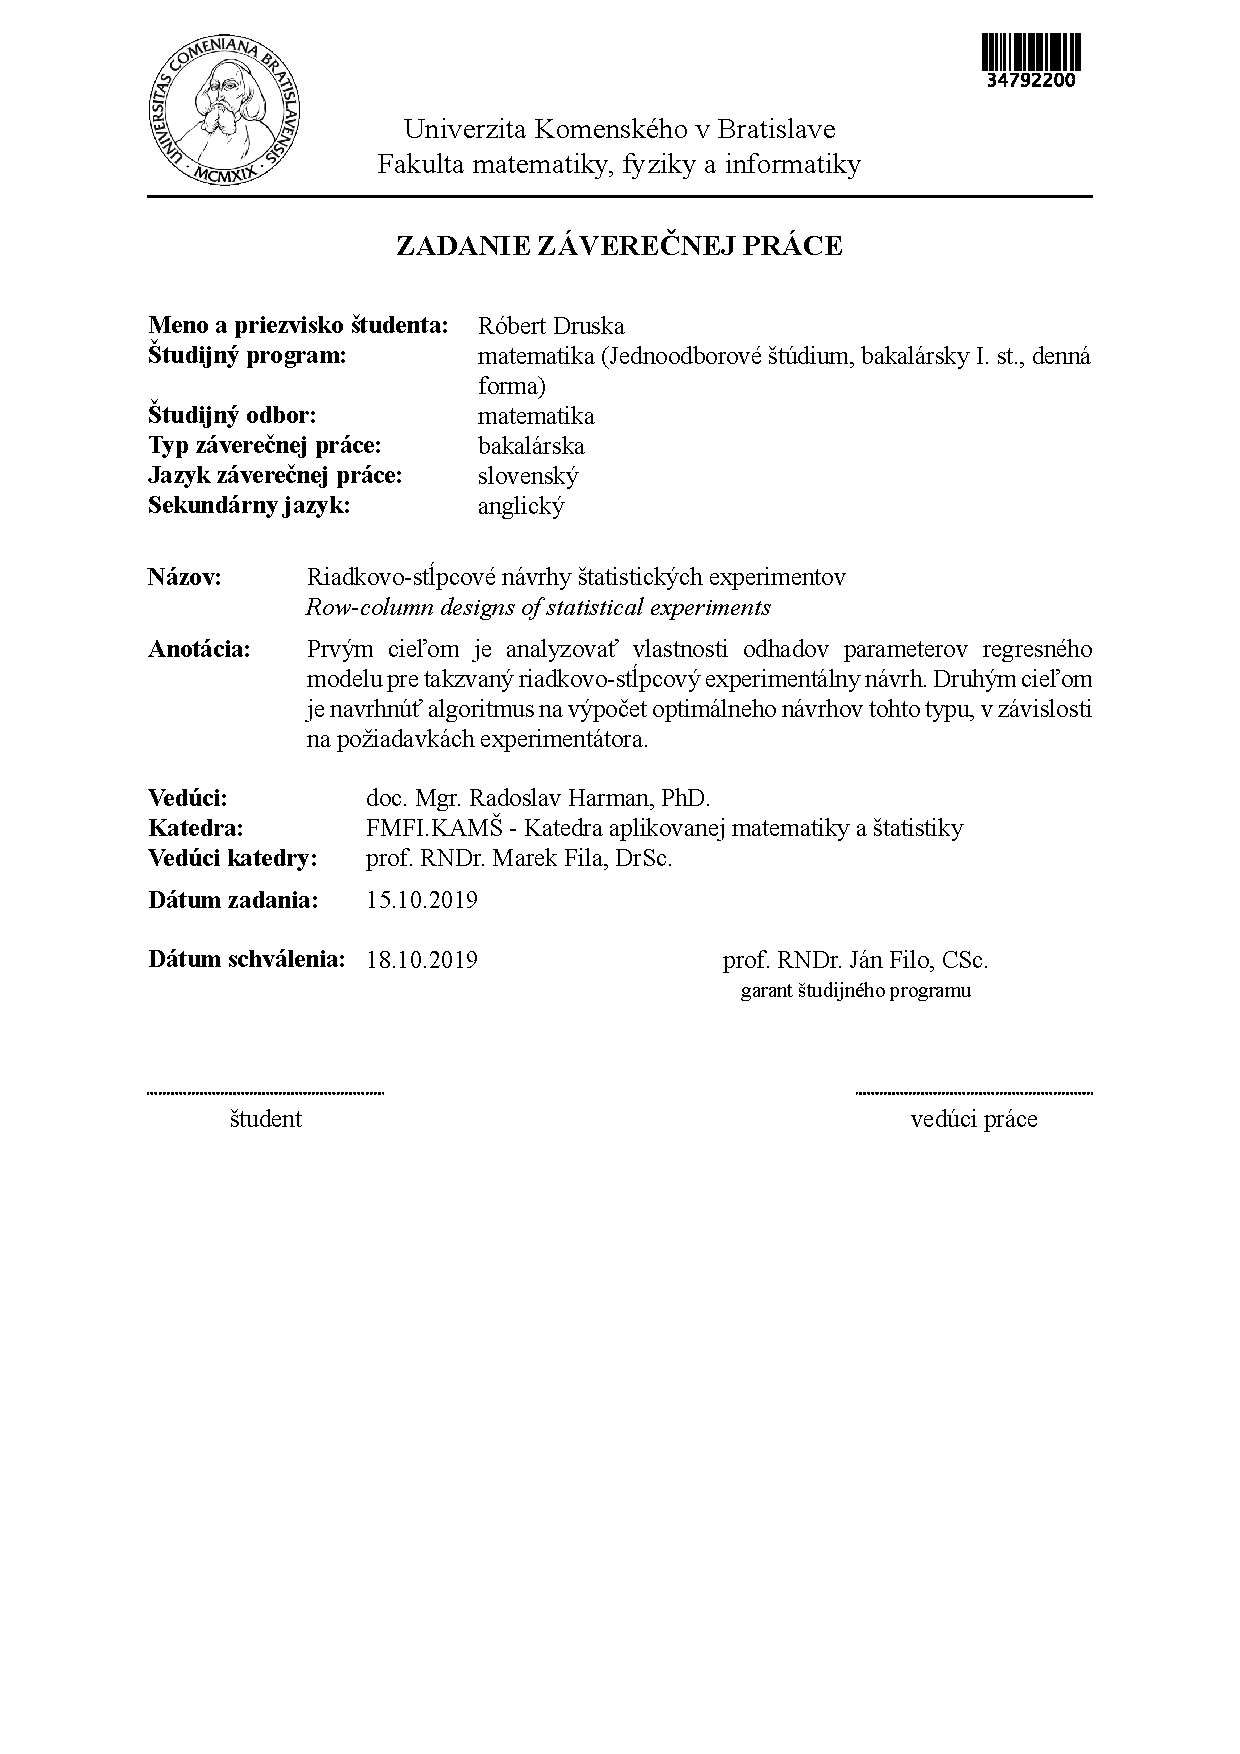
\includepdf[pages={1}, offset=25 -75]{zadanieRD.pdf}

  

\vglue0pt
\vfill
\thispagestyle{empty}
\paragraph{Poďakovanie}
TODO


  \newpage
  \thispagestyle{empty}
\section*{Abstrakt}
TODO

\begin{flushleft}
  \textbf{Kľúčové slová:} lineárny regresný model
\end{flushleft}

  \newpage
  \thispagestyle{empty}
\section*{Abstract}
Text abstraktu v svetovom jazyku je potrebný pre integráciu do medzinárodných informačných systémov (napr. The Network Digital Library of Theses and Dissertations).

{ \it Príklad  abstraktu (upravený):} \\
NOVÁK, Vladimír: Index Policies for Dynamic and Stochastic Problems [Bachelor
Thesis], Comenius University in Bratislava, Faculty of Mathematics, Physics and Informatics, Department of Applied Mathematics and Statistics; Supervisor: Mgr. Peter Jacko, PhD., Bratislava, 2011, 38p.

In our work we investigate the Whittle's index policy derivation framework in
the Markov decision process environment. We analyze a model for the multi-class job
scheduling for user with abandonment, with the objective of minimizing the total
holding costs and abandonment penalties. The work provides analytical solution of an
optimal index rule for the case in which there are 1 or 2 users in the system. For
the case with more users we use recent results from the multi-armed restless bandits
approach and derive a new simple index rule, denoted by AJN, for the idling and
the non-idling system. This index rule is proposed to use also in the system with
arrivals. We also report on an exhaustive study of numerical experiments for both
systems, in which we compare AJN index rule with  certain two standard  rules. This computational study suggests that our rule is almost always superior or equivalent to the other rules, and it is often optimal.

\begin{flushleft}
  \textbf{Keywords:} Markov Decision Process, Multi-armed Restless Bandit, Whittle Index, Index Policies,  Bellman Equation
\end{flushleft}
  \newpage \tableofcontents
  \setcounter{page}{7}
 % \newpage
 % \listoffigures
 % \newpage
 % \listoftables  
 % \newpage
 % \section*{Zoznam použitých symbolov} 
 %   
\begin{center}
{\it Toto je nepovinná kapitola. Pri malom počte symbolov nie je vhodné ju uvádzať.}

   \begin{tabular}{lp{.8\linewidth}}
     $|\boldsymbol{u}|$  & euklidovská norma vektora $\boldsymbol{u}$, $|\boldsymbol{u}|:=\sum_i u_i^2$ \\ [3pt]
     $\boldsymbol{r}$     & $\boldsymbol{r}:=(x,y,z)^{\rm{T}}$, resp. $\boldsymbol{r}:=(x_1,x_2,x_3)^{\rm{T}}$
   \end{tabular}
\end{center}

 %   \addcontentsline{toc}{section}{Zoznam použitých symbolov}
  \newpage

    \section*{Úvod}	          
    \markboth{ÚVOD}{ÚVOD}  
    \addcontentsline{toc}{section}{Úvod}
    
    
Hlavnú textovú časť záverečnej práce tvorí: úvod, jadro, záver, zoznam použitej literatúry.

V úvode autor stručne a výstižne charakterizuje stav poznania alebo praxe v oblasti, ktorá je predmetom záverečnej práce a oboznamuje čitateľa s významom, cieľmi a zámermi práce. Autor v úvode zdôrazňuje, prečo je práca dôležitá a prečo sa rozhodol spracovať danú tému. 


Rozsah úvodu je  1 až 1,5 strany.  Úvod spravidla obsahuje: 
\begin{itemize}
\item vymedzenie problematiky BP v kontexte aplikácií matematiky;
\item zdôvodnenie aktuálnosti danej témy;
\item charakterizácia stavu poznania alebo praxe (odkazy na literatúru);
\item nastolenie problémov, ktoré chce autor v BP riešiť;
\item vytýčenie cieľov, ktoré majú byť v BP dosiahnuté;
\item uvedenie použitých metód a postupov riešenia;
\item stručný náčrt obsahu jednotlivých kapitol BP.
\end{itemize}
 
	\section{Názov kapitoly}
\label{Nazovkapitoly}

Jadro je hlavná časť práce a jeho členenie je určené typom práce. Vo vedeckých a odborných prácach  má jadro spravidla tieto hlavné časti:
súčasný stav riešenej problematiky doma a v zahraničí,
\begin{itemize}
	\item cieľ práce,
	\item metodika práce a metódy skúmania,
	\item výsledky práce,
	\item diskusia. 
\end{itemize}

 
V časti Súčasný stav riešenej problematiky autor uvádza dostupné informácie a poznatky týkajúce sa danej témy. Zdrojom pre spracovanie sú aktuálne publikované práce domácich a zahraničných autorov. Podiel tejto časti práce má tvoriť približne 30 % práce.
Časť Cieľ práce jasne, výstižne a presne charakterizuje predmet riešenia. Súčasťou sú aj rozpracované čiastkové ciele, ktoré podmieňujú dosiahnutie cieľa hlavného. 

Časť Metodika práce a metódy skúmania spravidla obsahuje:
\begin{itemize}
	\item charakteristiku objektu skúmania,
	\item pracovné postupy, 
	\item spôsob získavania údajov a ich zdroje,
	\item použité metódy vyhodnotenia a interpretácie výsledkov,
	\item štatistické metódy. 
\end{itemize}

Výsledky práce a diskusia sú najvýznamnejšími časťami záverečnej práce. Výsledky (vlastné postoje alebo vlastné riešenie vecných problémov), ku ktorým autor dospel, sa musia logicky usporiadať a pri popisovaní sa musia dostatočne zhodnotiť. Zároveň sa komentujú všetky skutočnosti a poznatky v konfrontácii s výsledkami iných autorov. Ak je to vhodné, výsledky práce a diskusia môžu tvoriť aj jednu samostatnú časť a spoločne tvoria spravidla 30 až 40 \% záverečnej práce.

{\it V prípade čisto teoretických matematických prác je členenie jadra práce určené povahou problematiky. Zvyčajne prvé kapitoly oboznamujú s pojmami a výsledkami nevyhnutnými na pochopenie problematiky, nasleduje súčasný stav problematiky, ktorý logicky vyúsťuje do podrobného formulovania cieľov práce. Ďalšie kapitoly obsahujú vlastné výsledky práce.  Tieto majú byť formulované, popísané a odôvodnené tak, aby bolo možné ľahko overiť ich pravdivosť.}

\subsection{Názov podkapitoly}
\label{Nazovpodkapitoly}

Podkapitoly diplomovej práce slúžia na členenie textu bakalárskej práce s cieľom čo najväčšej prehľadnosti.


\subsubsection{Názov Tretia úroveň} 
Editujte svoju prácu v kapitolách a podkapitolách. Čísla kapitol a podkapitol (druhej a tretej úrovne) sa citujú v texte práce takto: 

... V kapitole \ref{Nazovkapitoly} sme už uviedli, že ...; ... pozri \ref{Ilustracie} ... atď. ...

Odporúčaný rozsah bakalárskej práce je 30 až 40 strán (54 000 až 72 000 znakov vrátane medzier). Do tohto rozsahu sa počíta len hlavný text, t. j. úvod, kapitoly, záver a zoznam použitej literatúry. Dôležitejší ako rozsah práce je kvalita práce a úroveň jej spracovania. Pri písaní je dôležité dbať na vyváženosť (proporcionálnosť) jednotlivých častí práce.):
\begin{itemize}
	\item úvod má spravidla  1 - 2 strany,
	\item teoreticko-metodologická časť tvorí spravidla jednu tretinu práce,
	\item ostatné kapitoly tvoria približne dve tretiny práce,
	\item záver má zvyčajne 1 - 2 strany.
\end{itemize}


 
	\section{...} 

	\newpage
  \section*{Záver}
    \addcontentsline{toc}{section}{Záver}
    \markboth{ZÁVER}{ZÁVER} 
    V závere je potrebné v stručnosti zhrnúť dosiahnuté výsledky vo vzťahu k stanoveným cieľom. 
Vzhľadom na to, že v práci už boli definované všetky potrebné pojmy, možno byť v závere omnoho konkrétnejší ako v úvode. Pri argumentovaní o splnení cieľov je žiaduce odkazovať na konkrétne očíslované alebo inak pomenované časti práce (odseky, algoritmy, metódy, vzorce, vzťahy, vety a ich dôkazy a pod.).

  
  \renewcommand{\refname}{Zoznam použitej literatúry}
  \begin{thebibliography}{99}

	\bibitem{kniha} Cooper, W. W., Seiford, L. M., Tone, K.: {\it Data Envelopment Analysis A Comprehensive Text with Models, Applications, References and DEA-Solver Software}, Kluwer Academic Publishers,  Boston, 2000
	
	\bibitem{skripta} Siebertová, Z.: {\it Prednášky z ekonometrie}, učebné texty, FMFI UK Bratislava, 2007, dostupné na internete (xx.xx.2017 {\tt - vložiť dátum stiahnutia z internetu}):  http://www.defm.fmph.uniba.sk/ludia/siebertova/ekonometria2011.html
	
	\bibitem{clanok} Ševčovič D., Halická M., Brunovský, P.: {\it DEA analysis for a large structured bank branch network}, Central European Journal of Operational Research 9 (2001), 329--342, dostupné na internete (xx.xx.2017  {\tt - vložiť dátum stiahnutia z internetu}):  http://www.iam.fmph.uniba.sk/institute/sevcovic/papers/cl19.pdf
\end{thebibliography}
%
%
%Zoznam použitej literatúry obsahuje úplný zoznam bibliografických odkazov. Rozsah tejto časti je daný množstvom použitých literárnych zdrojov, ktoré musia korešpondovať s citáciami použitými v texte.
%
%Jednotlivé položky v zozname bibliografických odkazov sa uvádzajú v abecednom poradí. Sú usporiadané podľa prvého prvku (údaja), za ktorým nasleduje rok vydania dokumentu. Za nim v prípade potreby nasledujú malé písmená, ktorými sa odlišujú odkazy s rovnakým prvým údajom a rokom vydania.  {\it V matematických prácach je zaužívaný iný spôsob citovania (tzv. modifikovaná metóda číselných odkazov), kde práce usporiadame podľa abecedy a každej práci priradíme poradové číslo uvedené v hranatých zátvorkách. Odkazujeme potom napr.  na prácu [7].}
%
%Pri citovaní je dôležitá etika citovania ako aj technika citovania. Etika citovania určuje spôsob dodržiavania etickej normy vo vzťahu k cudzím myšlienkam a výsledkom, ktoré sú obsiahnuté v iných dokumentoch a v použitej literatúre. Technika citovania, vyjadruje, či a ako správne, podľa normy STN ISO 690: 1998. Dokumentácia - Bibliografické odkazy - Obsah, forma a štruktúra., autor spája miesta v texte so záznamami o dokumentoch, ktoré sú v zozname bibliografických odkazov.
%
%Pri záverečných prácach odporúčame používať {\it modifikovanú metódu číselných odkazov. Možno však používať aj tu popísanú}  metódu citovania podľa prvého údaja (mena) a dátumu, pri ktorej sa v texte uvedie v zátvorkách prvý údaj (priezvisko autora, alebo prvé slovo z názvu) a rok vydania citovaného dokumentu. Ak sa prvý údaj už nachádza v rámci textu, v zátvorkách za nim sa uvedie len rok. V prípade potreby sa v zátvorkách uvedú za rokom aj čísla citovaných strán. Ak majú dva alebo niekoľko dokumentov ten istý prvý údaj a rovnaký rok, odlíšia sa malými písmenami (a, b, c, a pod.) za rokom vo vnútri zátvoriek. To isté sa urobí aj v zozname bibliografických odkazov.
%
%Príklady popisu dokumentov citácií podľa ISO 690 a ISO 690-2:
%
%V \TeX-u používame prostredie 
%\begin{verbatim}
%\begin{thebibliography}{99}
%  \bibitem{meno autora} ...
%  \bibitem{meno autora} ...
%	\bibitem{meno autora} ...
%\end{thebibliography}
%\end{verbatim}
%
%Podľa typu citovanej literatúry ju za \texttt{$\backslash$bibitem{meno autora}} píšeme v nasledovnom tvare:
%
%\subsection*{Knihy / Monografie} 
%Prvky popisu: \\
%Autor. rok vydania. Názov: podnázov (nepovinný). Poradie vydania. Miesto vydania: Vydavateľ, rok vydania. Rozsah strán. ISBN. 
%
%Ak sú traja autori oddeľujú sa pomlčkou. Ak je viac autorov ako traja uvedie sa prvý autor a skratka a kol. alebo et al. ak je to zahraničné dielo. Prvé vydanie sa v citačnom popise nemusí uvádzať.
%
%Príklady: 
%\begin{itemize}
%  \item OBERT, V. 2006. Návraty a odkazy. Nitra : Univerzita Konštantína Filozofa, 2006. 129 s. ISBN 80-8094-046-0.
%  \item{timko} TIMKO, J. - SIEKEL. P. - TURŇA. J. 2004. Geneticky modifikované organizmy. Bratislava: Veda, 2004. 104 s. ISBN 80-224-0834-4.
%	\item HORVÁT, J. a kol. 1999. Anatómia a biológia človeka. 1. vyd. Bratislava: Obzor, 1999. 425 s. ISBN 80-07-00031-5.
%\end{itemize}
%
%\subsection*{Článok v časopise}
%Prvky popisu: \\
%Autor. rok vydania. Názov. In Názov zdrojového dokumentu (noviny, časopisy). ISSN, rok, ročník, číslo zväzku, rozsah strán (strana od-do).
%
%Príklady:
%\begin{itemize}
%	\item STEINEROVÁ, J. 2000. Princípy formovania vzdelania v informačnej vede. In {\it Pedagogická revue}. ISSN 1335-1982, 2000, roč. 2, č. 3, s. 8-16.
%	\item BEŇAČKA, J. et al. 2009 A better cosine approximate solution to pendulum equation. In {\it International Journal of Mathematical Education in Science and Technology}. ISSN 0020-739X, 2009, vol. 40, no. 2, p. 206-215. 
%\end{itemize}
%
%\subsection*{Článok zo zborníka a monografie}
%Prvky popisu: \\
%Autor. rok vydania. Názov článku. In {\it Názov zborníka}. Miesto vydania : Vydavateľ, rok vydania. ISBN, Rozsah strán (strana od-do). 
%
%Príklady:
%\begin{itemize}
%	\item ZEMÁNEK, P. 2001 The machines for ''green works'' in vineyards and their economical evaluation. In {\it 9th International Conference: proceedings}. Vol. 2. {\it Fruit Growing and viticulture}. Lednice : Mendel University of Agriculture and Forestry, 2001. ISBN 80-7157-524-0, p. 262-268.
%	\item BOĎOVÁ, M. et al. 1990. An introduction to algorithmic and cognitive approaches for information retrieval. In 18. Informatické dni: sborník referátů z mezinárodní vědecké konference o současných poznatcích informačních a komunikačních technologiích a jejich využití. Praha : Univerzita Karlova, 1990. ISBN 80-01-02079-7. s. 17-28.
%\end{itemize}
%
%
%\subsection*{Elektronické dokumenty - monografie}
%Prvky popisu: \\
%Autor. rok vydania. {\it Názov} [Druh nosiča]. Vydanie. Miesto vydania: Vydavateľ, dátum vydania. Dátum aktualizácie. [Dátum citovania]. Dostupnosť a prístup. ISBN.
%
%Príklad:
%\begin{itemize}
%	\item SPEIGHT, J. G. 2005. {\it Lange's Handbook of Chemistry}. [online]. London : McGraw-Hill, 2005. 1572 p. [cit. 2009.06.10.] Dostupné na internete:  <http://www.knovel.com/web/portal/basic\_search/display?\_EXT\_KNOVEL\\
%	\_DISPLAY\_bookid$=$1347\&\_EXT\_KNOVEL\_DISPLAY\_fromSearch$=$true\&\_ \\
%	EXT\_KNOVEL\_DISPLAY\_searchType$=$basic>. ISBN 978-1-60119-261-5.
%\end{itemize}
%	
%\subsection*{Články v elektronických časopisoch a iné príspevky}
%Prvky popisu: \\
%Autor. rok vydania. Názov. In {\it Názov časopisu}. [Druh nosiča]. Rok vydania, ročník, číslo [dátum citovania]. Dostupnosť a prístup. ISSN. 
%
%Príklad:
%\begin{itemize}
%	\item HOGGAN, D. Challenges, Strategies, and Tools for Research Scientists. In {\it Electronic Journal of Academic and Special Librarianship} [online]. 2002, vol. 3, no. 3 [cit. 2003-01-10]. Dostupné na internete: <http://southernlibrarianship.icaap.org/content/v03n03/Hoggan\_d01.htm>. ISSN 1525-321X.
%\end{itemize}
%
%\subsection*{Príspevok v zborníku na CD-ROM}
%Prvky popisu: \\
%Autor. rok vydania. Názov. In {\it Názov zborníka} [Druh nosiča]. Miesto vydania : Vydavateľ, rok vydania,  rozsah strán (strana od-do). ISBN.
%
%Príklad:
%\begin{itemize}
% 	\item ZEMÁNEK, P. The machines for ''green works'' in vineyards and their economical evaluation. In {\it 9th International Conference: proceedings}. Vol. 2. Fruit Growing and viticulture [CD-ROM]. Lednice : Mendel University of Agriculture and Forestry, 2001, p. 262-268. ISBN 80-7157-524-0.
%\end{itemize}
%
%\subsection*{Vedecko-kvalifikačné práce}
%Prvky popisu: \\
%Autor. rok vydania. Názov práce : označenie druhu práce (dizertačná, doktorandská). Miesto vydania : Názov vysokej školy. Rok vydania. Rozsah strán.
%
%Príklad:
%\begin{itemize}
%	\item MIKULÁŠIKOVÁ, M. 1999. Didaktické pomôcka pre praktickú výučbu na hodinách výtvarnej výchovy pre 2. stupeň základných škôl : diplomová práca. Nitra: UKF, 1999. 62 s.
%\end{itemize}
%
%
%\subsection*{Výskumné správy}
%Prvky popisu: \\
%Autor. Rok vydania. {\it Názov práce} : druh správy (VEGA, priebežná správa). Miesto vydania : Názov inštitúcie, rok vydania. Rozsah strán.
%
%Príklad:
%\begin{itemize}
%	\item BAUMGARTNER, J. a kol. 1998 {\it Ochrana a udržiavanie genofondu zvierat, šľachtenie zvierat}: výskumná správa. Nitra : VÚŽV, 1998. 78 s.
%\end{itemize}
%
%\subsection*{Normy}
%Popis prvku: \\
%Označenie a číslo normy. Rok vydania (nie rok schválenia, alebo účinnosti): Názov normy.
%
%Príklad:
%\begin{itemize}
%	\item STN ISO 690:1998 Dokumentácia - Bibliografické odkazy - Obsah, forma a štruktúra.
%\end{itemize}
  
	\newpage
  \appendix
  \section*{Príloha A} 
    \addcontentsline{toc}{section}{Príloha A}
    \markboth{Príloha A}{Príloha A}
    \renewcommand{\thesection}{A.\arabic{section}}
\renewcommand{\theequation}{A.\arabic{equation}}
\renewcommand{\thefigure}{A.\arabic{figure}}
\setcounter{equation}{0}

\textbf{Malá násobilka}
  \hspace{15pt}
  \begin{align}
      1\times2 = 3
  \end{align}

    %\begin{comment}
%\end{comment}
\end{document}
